\documentclass{article}
\usepackage{graphicx}
\usepackage[margin=1in]{geometry}
\usepackage[double spacing]{set space}
\begin{document}
\section{Chapter 1}
\subsection{Introduction}
Astronomy is the oldest of the natural sciences, the study of the celestial objects,their positions, and characteristics. Astrophysics is the application ofthe Laws of Physics to understand Astronomy. In early times Astronomy only comprised of the observations of the motion of visible celestial objects, but with the passage of time, questions about the nature of the universe started to originate. Early studies only considered the Solar system but with the discovery of telescope scientists realized that there is more to the universe than just that. Now, in the era of modern Astronomy, scientists have found many astounding phenomenon happening in outer space. [1]
The following research includes a study of the motion of a spiral galaxy namely Andromeda. The analysis of the motion will be done by studying the rotation curve of the specified galaxy. I will develop a set of calculations including computational work, that will prove us that the solution of the Missing Mass Problem can be found without invoking Dark Matter. 
The first chapter of this thesis introduces the basic concepts that are the basis of the following research.
((written with progress)) 

\subsection{Evolution of the Universe}
 The origin and evolution of the Universe is proposed by the widely accepted Big Bang Theory, according to which the universe was created as a consequence of giant explosion of very dense and hot matter. After the explosion it started to expand and cool down, this cooling down resulted in the formation of elements and then in the formation of planets, stars, galaxies and various celestial objects. [2]
 
\subsection{Missing Mass Problem}
When the scientists studied the motion of the objects in the Solar system they fell right into the realms of Newtonian laws of kinematics. There was no question in these Laws until the scientists studied the large scale structures such as galaxies or cluster of galaxies. This was first observed by Jan Hendrick Oort in 1932, when he noticed that stars in the solar neighborhood moved faster than expected. In 1939, Horace Babcock measured the rotation curve to Andromeda Galaxy which resulted in the increasing mass to luminosity ratio. [3] Similarly, in 1959 Louise Volders demonstrated that the spiral galaxy M33 does not spin according to the Keplerian Dynamics. [4] The Rotation Curves give us the information of change in velocity as we move away from the center of a system. There were two conclusions drawn from such errors, that either our understanding of the Gravity is not quite right, in the case when we study large scale structures or there is some hidden matter that is providing enough force to these structures to move with certain accelerations.

\subsection{Dark Matter vs. MOND}
[7]   In 1933 Fritz Zwicky invoke the dark matter as a solution to this mass discrepancy problem by studying eight Coma galaxies. He calculated mass to light ratios of these galaxy and concluded that 90 percent of the mass that had been responsible for the observed ratio, was missing. The other method to find about missing mass was to study the rotational velocities of galaxies. And it was assumed that the stars in the galaxies will follow the Kepler's law like the planets in the solar system, i.e. their velocities will show a decline as moving through the radius. So it was assumed that there is some invisible matter affecting their motion. That matter was named as Dark Matter.
[8][5][6] The mass discrepancy observed in the stellar systems only happens when the acceleration of gravity falls below a fix value i.e.
$a_{0}= 1.2x10^-8 cm/s^2$.[9] In 1983, Mordehai Milgrom proposed a modification in the Newtons Dynamics that explains many properties of galaxies without  the need of non baryonic dark matter. It is also effective in describing the dynamics of galaxies and galaxy clusters and within some approximations, gravitational lensing. [10][11] MOND and Dark Matter give conceptually different but operationally equivalent description of cosmic phenomenon.

\subsection{work plan}
 This research is based on the work of Milgrom for solving the Missing Mass Problem. It focuses on calculation of Milgrom's constant to create an expected rotation curve without the mass descrepancy. 
(still to work)

\section{Chapter 2}
\subsection{Modified Newtonian Dynamics (MOND) [6]}
MOND is a numeric way of calculating the missing mass or the factor that is causing that problem   It relates MOND acceleration 'a' to Newtonian acceleration $a_{N}$ by the following formula \begin{equation}
 a_{N}= a\mu(\frac{a}{a_{N}})
\end{equation}
where $a_{N} = 1.2×10-8  cms-2$  is a constant of physics. 
The interpolation function $\mu (a/a0)$ shows asymptotic behaviour $\mu=1$ when $a>> a0$,  which retrieves the Newtonian expression in strong field regime. And for $a << a0$ with these assumptions gives us the following expression, 
\begin{equation}
a= \sqrt{a_{N}a_{0}}= \frac{\sqrt{GMa_{0}}}{r}
\end{equation} 
different functions are used for $\mu$, currently most used function is :
\begin{equation}
(\frac{a}{a_{0}}) = \frac{\frac{a}{a_{0}}}{\sqrt{1+(\frac{a}{a_{0}})^2}•}
\end{equation} 
it works well for galactic rotation and solving for a, it gives 
\begin{equation}
a= a_{N}(\frac{1}{2}+\frac{1}{2\sqrt{1+(\frac{2a_{0}}{a_{N}})^2}})^\frac{1}{2}
\end{equation}
the above expression allows us to calculate the MOND acceleration provided Newtonian gravity is known. 
\subsection{Area of Study}
  MOND has been tested successfully on spiral galaxies, so for this research we choose our nearest spiral galaxy i.e. Andromeda Galaxy.(work it out)
  \subsection*{Andromeda Galaxy}
  Andromeda, M31 or NGC 224 is the nearest spiral galaxy to Milky Way.  (still to work)
\subsection{Distance to the Galaxy}
The stars and galaxies are far apart from Earth, these distances can vary from a few parsecs to kilo and mega parsecs. It is important to calculate the distances in order to determine further properties of these objects. There are different techniques to calculate distances, that astronomers have developed. 
A few of them are listed below:
\subsection*{Standard Candles[12]}
 Cepheid variable stars are used to as cosmic distance ladders to measure distances. Cepheid variable stars are a part of star cycle, formed when a giant red star is about to die. These stars expand and contract, changing their brightness from lighter to dimmer.  They change their brightness in regular intervals of 1 to 70 days. And the relation between the time interval and apparent magnitude gives us distances by the following equation:
 \begin{equation}
 d= 10^{\frac{(m-M+5)}{5}}
 \end{equation}
where \textbf{m} is the apparent magnitude and \textbf{M} is the absolute magnitude.
\subsection*{Binary Stars 13}
Binary stars system is the one which have two stars orbiting around a center of mass, hence they are gravitationally bound to each other. Almost \textbf{85} percent of the stars are binary in nature. The orbital periods and distances of these system vary enormously. Some times they are so close that they can transfer matter and others can be separated a few hundreds light years and have period of hundreds of year. Following are the types of binary stars systems:
\begin{itemize}
\item \textbf{Visual Binaries} [14]

  Some binary systems are close to Earth and have a significantly large distances between each    other, so they can be visualized individually in a telescope. These systems are known as visual binaries. 
\item \textbf{Spectroscopic Binaries }

Most binary systems are too far to be resolved by telescopes, so they are detected by the Doppler Shifts in their spectral lines. Such systems are spectroscopic binary system. The two stars appear to be moving towards and away from us. So the one moving towards us is blue shifted while the one moving away is red shifted.


\item\textbf{ Astrometric Binaries}

The Binary stars sometimes are too far or two close. Sometimes it is hard to distinguish between the two stars in the system, such systems of binary stars are known as Astrometric binary stars.
[http://csep10.phys.utk.edu/astr162/lect/binaries/astrometric.html]

\item \textbf{Eclipsing Binaries}
[http://www.physics.sfasu.edu/astro/ebstar/ebstar.html]
The type of variable stars, that appear as single point of light , but due to brightness variation and spectroscopic observations we say they are two stars in close orbit around each other. 
These binary systems give the best estimates of distances.
The graph of brightness versus time is known as Light curve of eclipsing binaries. Time is expressed as phase, and the unit of phase is orbital period. The brightness is measured as magnitude of the stars. 

\begin{figure}
\centering
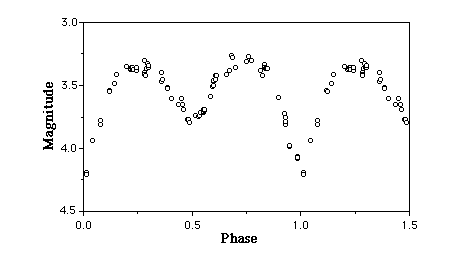
\includegraphics[scale=0.5]{LC}
\caption{Photometry of Beta Lyrae in 1992-1993}
\end{figure}

\end{itemize}
  

\end{document}
